% !TeX spellcheck = en_US
% !TeX root = ./0_article.tex

\section{How to perform BBI in a better way}
	\subsection{BBI platforms in the state of the art}
		In the first place, we will analyze, from a theoretical perspective, a typical BBI platform.
		To do so, we created simple platform models allowing to highlight the major limiting factors of such platforms.
		% !TeX spellcheck = en_US
% !TeX root = ./0_article.tex

\begin{figure}[h]
	\centering
	\subfloat[][Typical]{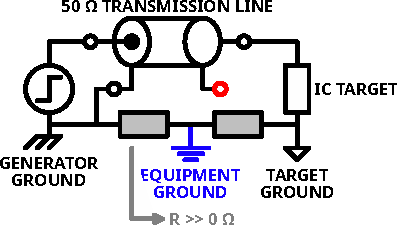
\includegraphics[width=0.5\columnwidth]{./figures/state-of-the-art-platform.pdf}}
	\subfloat[][Improved]{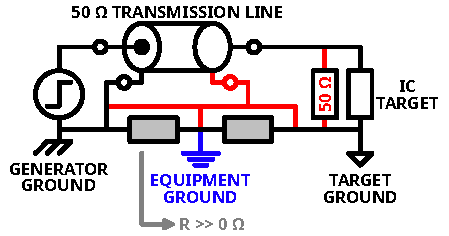
\includegraphics[width=0.5\columnwidth]{./figures/s-bbi-better.pdf}}
	\caption{Simple models of a typical (a) and an improved (b) BBI setup.}
	\label{bbi_setups}
\end{figure}

		The typical platform model is described in Fig. \ref{bbi_setups}.a and shows the main components making a BBI platform such as:
		\begin{itemize}
			\item The voltage pulse generator;
			\item The transmission line;
			\item The grounding installation;
			\item The IC target.
		\end{itemize}
		In addition to this, the schematic shows some important flaws we are going to address.
		
		While this is not always the case, voltage pulse generators are typically specified to be loaded with a 50 \textOmega\ load, or more generally with a fixed load.
		When performing BBI, the backside of the IC is electrically connected to the generator output.
		Therefore, outside of luck alone, it is very rare that the impedance presented by the IC to the generator perfectly matches the required one.
		It implies that the generator will be, most of the time, out of specifications, and that the conditions will vary depending on the chosen IC and the location of the BBI probe.
		This can lead to issues such as errors in the set-point voltage and pulse width, and ringing in the transmission line.
		It then represents a first flaw to the typical approach.
		
		Then, there is the grounding installation.
		The model presents a non-ideal but simple platform grounding.
		The reference, used by the oscilloscope and the main computer, is represented in blue and called "equipment ground".
		Ideally, every ground on the platform is connected to this reference with a very low impedance interconnection.
		However, depending on the hardware used, it may greatly vary from one platform to another.
		In the model, the secondaries generator and target grounds are connected to the reference thanks to vastly imperfect interconnections, whose impedance is significantly higher than zero.
		This mainly lead to set-point errors due to shifts in the voltage pulse amplitude.
		Therefore, it limits the inter-platform repeatability of BBI experiments.
	
	\subsection{Improvements proposed}
		To circumvent the previously introduced limitations, we propose two corrections to generalize the platforms and improve the repeatability.
		
		First, let us talk about the improper grounding,
		Alleviating this issue is fairly straightforward.
		To do so, we propose to choose a reference, such as the equipment ground, and bypass all the grounds with low-impedance interconnections from this reference, as proposed in red in Fig. \ref{bbi_setups}.b.
		
		Then, concerning the impedance mismatch of the generator, multiple solutions can be approached.
		The best solution would be to implement an adaptive impedance matching system with active feedback, able to measure in real-time the impedance seen by the generator.
		However, adopting such a method is costly and long to set up in comparison to the next solution.
		Therefore, we propose a much simpler approach.
		Since, most of the time, the impedance presented by the IC on its backside is in the order of 1 k\textOmega\, approaching the 50 \textOmega\ expected by the generator can be done by connecting in parallel to the IC a 50 \textOmega\ resistor, as it is shown in the schematic in Fig. \ref{bbi_setups}.b.
		
	\subsection{Platform improvements in practice}
		% !TeX spellcheck = en_US
% !TeX root = ./0_article.tex

\begin{figure}[h]
	\centering
%	\subfloat[][Typical]{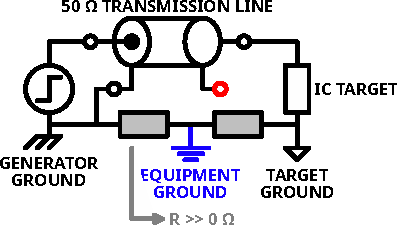
\includegraphics[width=0.5\columnwidth]{./figures/state-of-the-art-platform.pdf}}
%	\subfloat[][Improved]{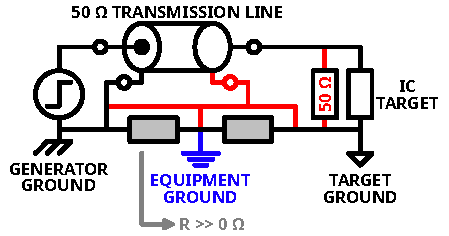
\includegraphics[width=0.5\columnwidth]{./figures/s-bbi-better.pdf}}
	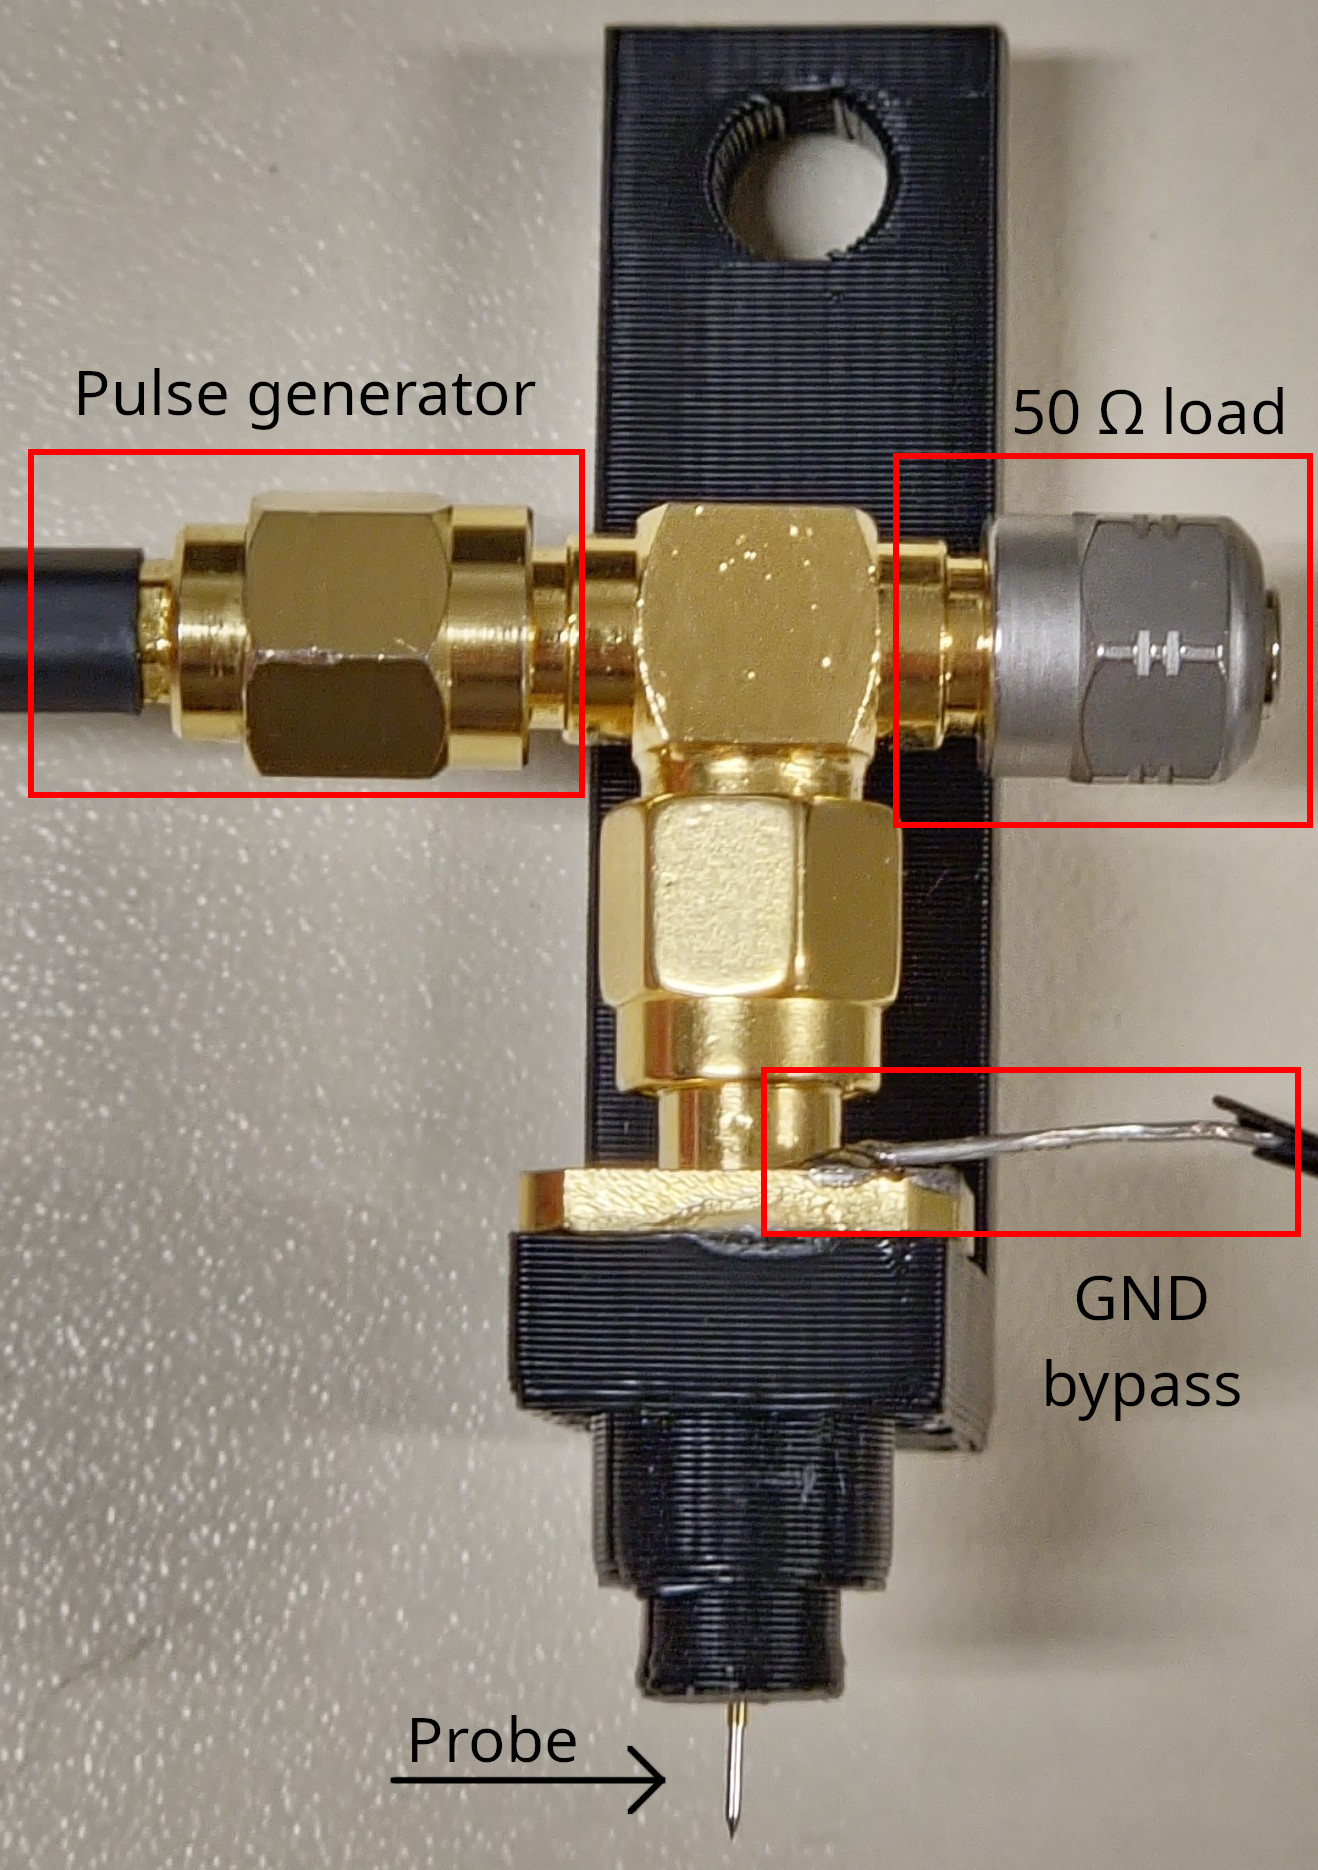
\includegraphics[width=0.40\columnwidth]{./figures/sondeGndSource.jpg}
	\caption{Impedance matching in practice.}
	\label{imp_match_real}
\end{figure}

		The proposed solution concerning the approximate impedance matching is shown in Fig. \ref{imp_match_real}.
		The picture shows the BBI probe with a compensation load connected in parallel.
		To show the actual interests of these improvements, let us analyze signals from an actual platform.
		
		We will compare before and after results and analyze the differences made by these improvements.
		To that end, we set up simple experiments consisting in injecting a voltage pulse into our IC target, measuring the voltage pulse at the probe and the current in the IC.
		% !TeX spellcheck = en_US
% !TeX root = ./0_article.tex

\begin{figure}[h]
	\centering
	%	\subfloat[][Typical]{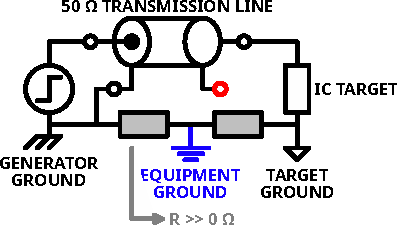
\includegraphics[width=0.5\columnwidth]{./figures/state-of-the-art-platform.pdf}}
	%	\subfloat[][Improved]{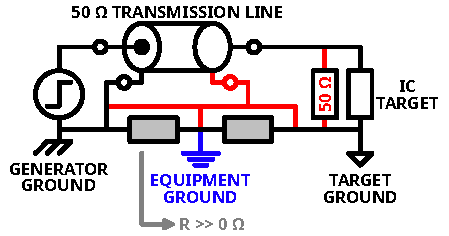
\includegraphics[width=0.5\columnwidth]{./figures/s-bbi-better.pdf}}
	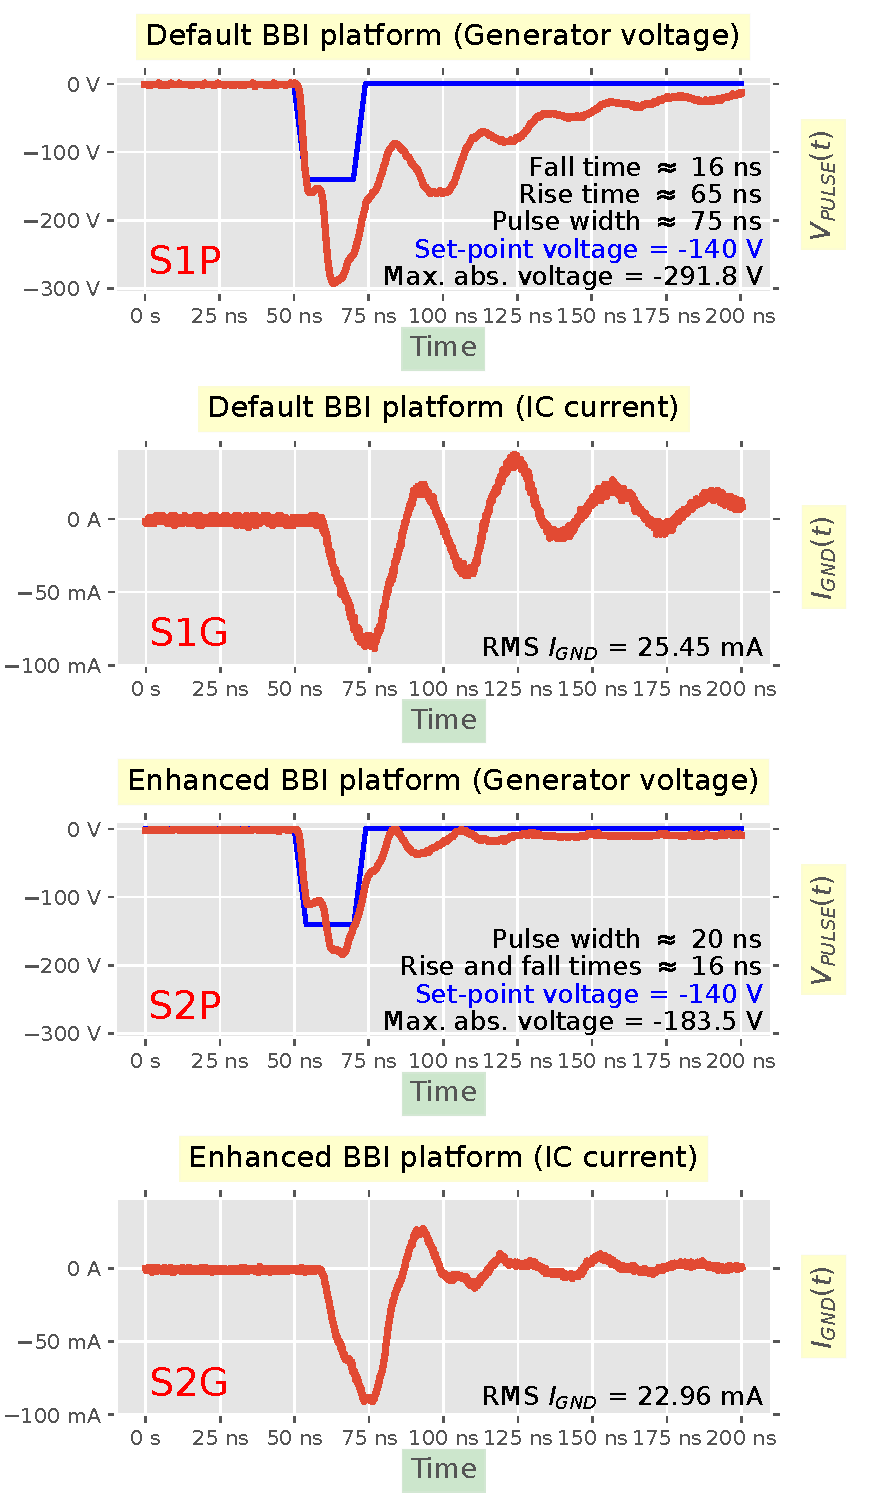
\includegraphics[width=\columnwidth]{./figures/realPulsesComparisons.pdf}
	\caption{Platform improvements in practice}
	\label{actual_imp}
\end{figure}

		Fig. \ref{actual_imp} presents the waveform results of such experiments.
		The figure is split in two main parts, the top row shows the results before the improvements, and the bottom row shows the results after the improvements.
		The experimental conditions are the following:
		\begin{itemize}
			\item Voltage pulse amplitude = -140 V;
			\item Voltage pulse width = 20 ns;
			\item Rise and fall times = 4 ns.
		\end{itemize}
		
		The waveform S1P shows in blue the ideal waveform according to the generator settings and in red the measured waveform.
		In addition to this are annotated some noteworthy values.
		The first thing to notice here is the obvious undershoot of about -110 \% under the set-point.
		It is far from being desirable when performing fault injection as the voltage amplitude is of great importance when considering the method effects on the IC.
		Furthermore, the pulse width is 275 \& higher than the set-point, measuring 75 ns instead of 20 ns.
		It is an additional issue as it annihilates the accuracy needed in this context, and leads to longer pulses injected into the IC and potentially more energy than required.
		Additionally, the rise and fall times are also 4 to 16 times higher than expected.
		Eventually, we can notice damped oscillations, probably the proof of ringing in the transmission line.
		
		Then, the waveform S1G, associated with the previous one, shows the IC ground current.
		Here, the damped oscillations are more clearly visible, in addition to the much longer than expected pulse duration.
		The RMS value of the injected current measures around 25 mA.
		
		Afterwards, 
	
%	Three main flaws lie in the platform in its current state:
%	\begin{itemize}
%		\item The pulse generator
%	\end{itemize}
